\chapter{Mastering the grammar}\label{cha:mastery}

\section{Introduction}

You can choose to use just \texttt{qplot()}, without any understanding
of the underlying grammar, but if you do you will never be able to
unlock the full power of ggplot. By learning more about the grammar and
its components, you will be able to create a wider range of plots, as
well as being able to combine multiple sources of data, and customise to
your heart's content. You may want to skip this chapter in a first
reading of the book, returning when you want a deeper understanding of
how all the pieces fit together.

This chapter describes the theoretical basis of \textbf{ggplot}: the
layered grammar of graphics. The layered grammar is based on Wilkinson's
grammar of graphics (Wilkinson 2005), but adds a number of enhancements
that help it to be more expressive and fit seamlessly into the R
environment. The differences between the layered grammar and Wilkinson's
grammar are described fully in (Wickham 2008), and a guide for
converting between \texttt{GPL} (the encoding of the grammar used in
\texttt{SPSS}) and \textbf{ggplot} is included in
\hyperref[cha:translating]{translating}. In this chapter you will learn
a little bit about each component of the grammar and how they all fit
together. The next chapters discuss the components in more detail, and
provide more examples of how you can use them in practice.

The grammar is useful for you both as a user and as a potential
developer of statistical graphics. As a user, it makes it easier for you
to iteratively update a plot, changing a single feature at a time. The
grammar is also useful because it suggests the high-level aspects of a
plot that \emph{can} be changed, giving you a framework to think about
graphics, and hopefully shortening the distance from mind to paper. It
also encourages the use of graphics customised to a particular problem,
rather than relying on generic named graphics.

As a developer, the grammar makes it much easier to add new capabilities
to \textbf{ggplot}. You only need to add the one component that you
need, and you can continue to use all of the other existing components.
For example, you can add a new statistical transformation, and continue
to use the existing scales and geoms. It is also useful for discovering
new types of graphics, as the grammar effectively defines the parameter
space of statistical graphics.

This chapter begins by describing in detail the process of drawing a
simple plot. \hyperref[sec:simple-plot]{Building a scatterplot} starts
with a simple scatterplot, then \hyperref[sec:complex-plot]{Adding
complexity} makes it more complex by adding a smooth line and faceting.
While working through these examples you will be introduced to all six
components of the grammar, which are then defined more precisely in
\hyperref[sec:components]{Components of the layered grammar}. The
chapter concludes with \hyperref[sec:data-structures]{Data structures},
which describes how the various components map to data structures in R.

\section{Fuel economy data}\label{sec:fuel-economy-data}

Consider the fuel economy dataset, \texttt{mpg}, a sample of which is
illustrated in Table \ref{tbl:mpg}. It records make, model, class,
engine size, transmission and fuel economy for a selection of US cars in
1999 and 2008. It contains the 38 models that were updated every year,
an indicator that the car was a popular model. These models include
popular cars like the Audi A4, Honda Civic, Hyundai Sonata, Nissan
Maxima, Toyota Camry and Volkswagen Jetta. This data comes from the EPA
fuel economy website, \url{http://fueleconomy.gov}.
\index{Data!mpg@\texttt{mpg}}

\begin{table}[ht]
\centering
\begin{tabular}{llrrrlrrll}
  \hline
manufacturer & model & displ & year & cyl & drv & cty & hwy & fl & class \\ 
  \hline
audi & a4 & 1.80 & 1999 &   4 & f &  18 &  29 & p & compact \\ 
  audi & a4 & 1.80 & 1999 &   4 & f &  21 &  29 & p & compact \\ 
  audi & a4 & 2.00 & 2008 &   4 & f &  20 &  31 & p & compact \\ 
  audi & a4 & 2.00 & 2008 &   4 & f &  21 &  30 & p & compact \\ 
  audi & a4 & 2.80 & 1999 &   6 & f &  16 &  26 & p & compact \\ 
  audi & a4 & 2.80 & 1999 &   6 & f &  18 &  26 & p & compact \\ 
  audi & a4 & 3.10 & 2008 &   6 & f &  18 &  27 & p & compact \\ 
  audi & a4 quattro & 1.80 & 1999 &   4 & 4 &  18 &  26 & p & compact \\ 
  audi & a4 quattro & 1.80 & 1999 &   4 & 4 &  16 &  25 & p & compact \\ 
  audi & a4 quattro & 2.00 & 2008 &   4 & 4 &  20 &  28 & p & compact \\ 
   \hline
\end{tabular}
\caption{The first 10 cars in the \texttt{mpg} dataset, included in the ggplot2 package.  \texttt{cty} and \texttt{hwy} record miles per gallon (mpg) for city and highway driving, respectively, and \texttt{displ} is the engine displacement in litres.} 
\label{tbl:mpg}
\end{table}

This dataset suggests many interesting questions. How are engine size
and fuel economy related? Do certain manufacturers care more about
economy than others? Has fuel economy improved in the last ten years? We
will try to answer the first question and in the process learn more
details about how the scatterplot is created.

\hyperdef{}{sec:simple-plot}{\section{Building a
scatterplot}\label{sec:simple-plot}}

Consider Figure \ref{fig:mpgg}, one attempt to answer this question. It
is a scatterplot of two continuous variables (engine displacement and
highway mpg), with points coloured by a third variable (number of
cylinders). From your experience in the previous chapter, you should
have a pretty good feel for how to create this plot with
\texttt{qplot()}. But what is going on underneath the surface? How does
\textbf{ggplot} draw this plot? \index{Scatterplot!principles of}

\begin{Shaded}
\begin{Highlighting}[]
\KeywordTok{qplot}\NormalTok{(displ, hwy, }\DataTypeTok{data =} \NormalTok{mpg, }\DataTypeTok{colour =} \KeywordTok{factor}\NormalTok{(cyl))}
\end{Highlighting}
\end{Shaded}

\begin{figure}

{\centering \includegraphics[width=\linewidth]{figures/masterympgg-1} 

}

\caption{A scatterplot of engine displacement in litres (displ) vs. average highway miles per gallon (hwy).  Points are coloured according to number of cylinders.  This plot summarises the most important factor governing fuel economy: engine size.\label{fig:mpgg}}
\end{figure}

\subsection{Mapping aesthetics to data}

What precisely is a scatterplot? You have seen many before and have
probably even drawn some by hand. A scatterplot represents each
observation as a point, positioned according to the value of two
variables. As well as a horizontal and vertical position, each point
also has a size, a colour and a shape. These attributes are called
\textbf{aesthetics}, and are the properties that can be perceived on the
graphic. Each aesthetic can be mapped to a variable, or set to a
constant value. In Figure \ref{fig:mpgg} \texttt{displ} is mapped to
horizontal position, \texttt{hwy} to vertical position and \texttt{cyl}
to colour. Size and shape are not mapped to variables, but remain at
their (constant) default values. \index{Mappings}

Once we have these mappings we can create a new dataset that records
this information. Table \ref{tbl:mapping} shows the first 10 rows of the
data behind Figure \ref{fig:mpgg}. This new dataset is a result of
applying the aesthetic mappings to the original data. We can create many
different types of plots using this data. The scatterplot uses points,
but were we instead to draw lines we would get a line plot. If we used
bars, we'd get a bar plot. Neither of those examples makes sense for
this data, but we could still draw them, as in Figure
\ref{fig:other-geoms}. In ggplot, we can produce many plots that don't
make sense, yet are grammatically valid. This is no different than
English, where we can create senseless but grammatical sentences like
the angry rock barked like a comma.

\begin{table}[ht]
\centering
\begin{tabular}{rrr}
  \hline
x & y & colour \\ 
  \hline
1.80 &  29 &   4 \\ 
  1.80 &  29 &   4 \\ 
  2.00 &  31 &   4 \\ 
  2.00 &  30 &   4 \\ 
  2.80 &  26 &   6 \\ 
  2.80 &  26 &   6 \\ 
  3.10 &  27 &   6 \\ 
  1.80 &  26 &   4 \\ 
  1.80 &  25 &   4 \\ 
  2.00 &  28 &   4 \\ 
   \hline
\end{tabular}
\caption{First 10 rows from \texttt{mpg} rearranged into the format required for a scatterplot.  This data frame contains all the data to be displayed on the plot.} 
\label{tbl:mapping}
\end{table}

\begin{Shaded}
\begin{Highlighting}[]
\KeywordTok{qplot}\NormalTok{(displ, hwy, }\DataTypeTok{data =} \NormalTok{mpg, }\DataTypeTok{colour =} \KeywordTok{factor}\NormalTok{(cyl), }\DataTypeTok{geom =} \StringTok{"line"}\NormalTok{) +}\StringTok{ }
\StringTok{  }\KeywordTok{theme}\NormalTok{(}\DataTypeTok{legend.position =} \StringTok{"none"}\NormalTok{)}
\KeywordTok{qplot}\NormalTok{(displ, hwy, }\DataTypeTok{data =} \NormalTok{mpg, }\DataTypeTok{colour =} \KeywordTok{factor}\NormalTok{(cyl), }\DataTypeTok{geom =} \StringTok{"bar"}\NormalTok{, }
  \DataTypeTok{stat =} \StringTok{"identity"}\NormalTok{, }\DataTypeTok{position =} \StringTok{"identity"}\NormalTok{) +}\StringTok{ }
\StringTok{  }\KeywordTok{theme}\NormalTok{(}\DataTypeTok{legend.position =} \StringTok{"none"}\NormalTok{)}
\end{Highlighting}
\end{Shaded}

\begin{figure}

{\centering \includegraphics[width=0.49\linewidth]{figures/masteryother-geoms-1} \includegraphics[width=0.49\linewidth]{figures/masteryother-geoms-2} 

}

\caption{Instead of using points to represent the data, we could use other geoms like lines (left) or bars (right).  Neither of these geoms makes sense for this data, but they are still grammatically valid.\label{fig:other-geoms}}
\end{figure}

Points, lines and bars are all examples of geometric objects, or
\textbf{geoms}. Geoms determine the ``type'' of the plot. Plots that use
a single geom are often given a special name, a few of which are listed
in Table \ref{tbl:named-plots}. More complex plots with combinations of
multiple geoms don't have a special name, and we have to describe them
by hand. For example, Figure \ref{fig:complex-plot} overlays a per group
regression line on the existing plot. What would you call this plot?
Once you've mastered the grammar, you'll find that many of the plots
that you produce are uniquely tailored to your problems and will no
longer have special names. \index{Named plots}

\begin{table}[ht]
\centering
\begin{tabular}{lll}
  \hline
Named plot & Geom & Other features \\ 
  \hline
scatterplot & point &  \\ 
  bubblechart & point & size mapped to a variable \\ 
  barchart & bar &  \\ 
  box-and-whisker plot & boxplot &  \\ 
  line chart & line &  \\ 
   \hline
\end{tabular}
\caption{A selection of named plots and the geoms that they correspond to.} 
\label{tbl:named-plots}
\end{table}

\begin{Shaded}
\begin{Highlighting}[]
\KeywordTok{qplot}\NormalTok{(displ, hwy, }\DataTypeTok{data =} \NormalTok{mpg, }\DataTypeTok{colour =} \KeywordTok{factor}\NormalTok{(cyl)) +}\StringTok{ }
\StringTok{  }\KeywordTok{geom_smooth}\NormalTok{(}\DataTypeTok{data =} \KeywordTok{subset}\NormalTok{(mpg, cyl !=}\StringTok{ }\DecValTok{5}\NormalTok{), }\DataTypeTok{method =} \StringTok{"lm"}\NormalTok{)}
\end{Highlighting}
\end{Shaded}

\begin{figure}

{\centering \includegraphics[width=\linewidth]{figures/masterycomplex-plot-1} 

}

\caption{More complicated plots don't have their own names. This plot takes Figure~\ref{fig:mpgg} and adds a regression line to each group. What would you call this plot?\label{fig:complex-plot}}
\end{figure}

\subsection{Scaling}

The values in Table \ref{tbl:mapping} have no meaning to the computer.
We need to convert them from data units (e.g., litres, miles per gallon
and number of cylinders) to physical units (e.g., pixels and colours)
that the computer can display. This conversion process is called
\textbf{scaling} and performed by scales. Now that these values are
meaningful to the computer, they may not be meaningful to us: colours
are represented by a six-letter hexadecimal string, sizes by a number
and shapes by an integer. These aesthetic specifications that are
meaningful to R are described in
\hyperref[cha:specifications]{specifications}.
\index{Scales!introduction}

In this example, we have three aesthetics that need to be scaled:
horizontal position (x), vertical position (y) and colour. Scaling
position is easy in this example because we are using the default linear
scales. We need only a linear mapping from the range of the data to
\([0, 1]\). We use \([0, 1]\) instead of exact pixels because the
drawing system that \textbf{ggplot} uses, \textbf{grid}, takes care of
that final conversion for us. A final step determines how the two
positions (x and y) are combined to form the final location on the plot.
This is done by the coordinate system, or \textbf{coord}. In most cases
this will be Cartesian coordinates, but it might be polar coordinates,
or a spherical projection used for a map.

The process for mapping the colour is a little more complicated, as we
have a non-numeric result: colours. However, colours can be thought of
as having three components, corresponding to the three types of
colour-detecting cells in the human eye. These three cell types give
rise to a three-dimensional colour space. Scaling then involves mapping
the data values to points in this space. There are many ways to do this,
but here since \texttt{cyl} is a categorical variable we map values to
evenly spaced hues on the colour wheel, as shown in Figure
\ref{fig:colour-wheel}. A different mapping is used when the variable is
continuous. \index{Colour!wheel}

\begin{figure}[htbp]
  \centering
    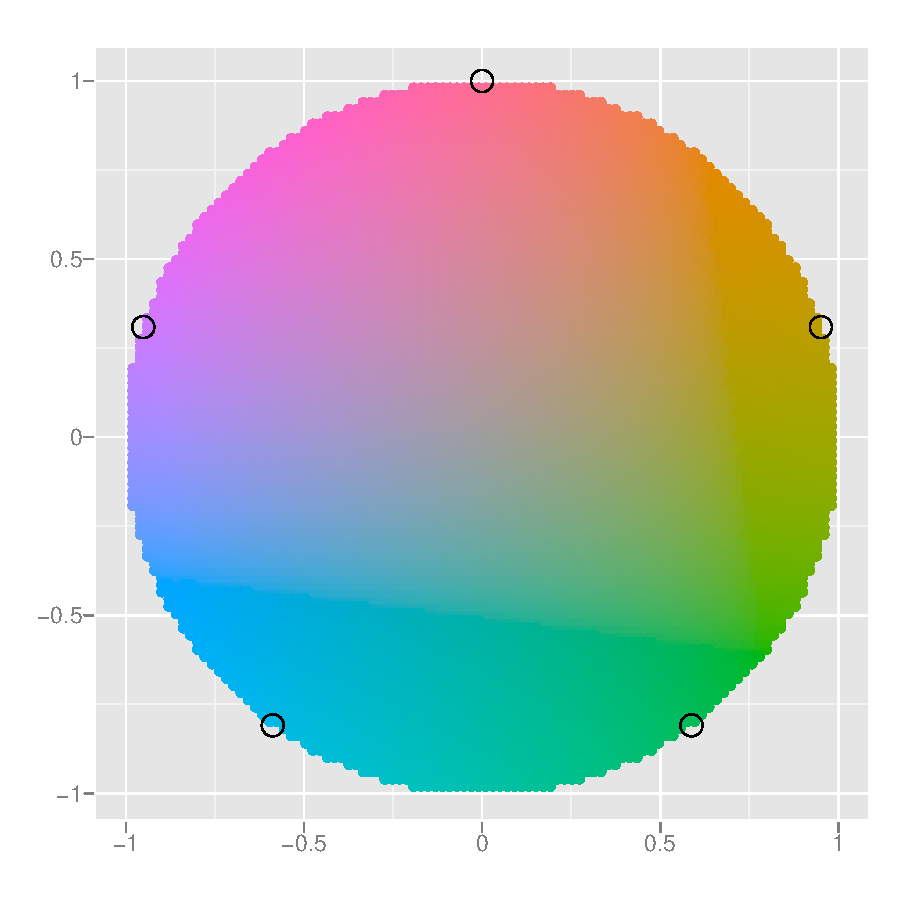
\includegraphics[width=3in]{diagrams/colour-wheel}
  \caption{A colour wheel illustrating the choice of five equally spaced colours. This is the default scale for discrete variables.}
  \label{fig:colour-wheel}
\end{figure}

The result of these conversions is Table \ref{tbl:scaled}, which
contains values that have meaning to the computer. As well as aesthetics
that have been mapped to variable, we also include aesthetics that are
constant. We need these so that the aesthetics for each point are
completely specified and R can draw the plot.

\definecolor{f8766d}{rgb}{0.972549019607843, 0.462745098039216, 0.427450980392157}
\definecolor{00bfc4}{rgb}{0, 0.749019607843137, 0.768627450980392}
\definecolor{c77cff}{rgb}{0.780392156862745, 0.486274509803922, 1}
\definecolor{7cae00}{rgb}{0.486274509803922, 0.682352941176471, 0}

\begin{table}[ht]
\centering
\begin{tabular}{lllrr}
  \hline
`x` & `y` & `colour` & `size` & `shape` \\ 
  \hline
0.037 & 0.531 & $\backslash$color\{f8766d\} $\backslash$\#F8766D & 1.00 & 19.00 \\ 
  0.037 & 0.531 & $\backslash$color\{f8766d\} $\backslash$\#F8766D & 1.00 & 19.00 \\ 
  0.074 & 0.594 & $\backslash$color\{f8766d\} $\backslash$\#F8766D & 1.00 & 19.00 \\ 
  0.074 & 0.562 & $\backslash$color\{f8766d\} $\backslash$\#F8766D & 1.00 & 19.00 \\ 
  0.222 & 0.438 & $\backslash$color\{00bfc4\} $\backslash$\#00BFC4 & 1.00 & 19.00 \\ 
  0.222 & 0.438 & $\backslash$color\{00bfc4\} $\backslash$\#00BFC4 & 1.00 & 19.00 \\ 
  0.278 & 0.469 & $\backslash$color\{00bfc4\} $\backslash$\#00BFC4 & 1.00 & 19.00 \\ 
  0.037 & 0.438 & $\backslash$color\{f8766d\} $\backslash$\#F8766D & 1.00 & 19.00 \\ 
  0.037 & 0.406 & $\backslash$color\{f8766d\} $\backslash$\#F8766D & 1.00 & 19.00 \\ 
  0.074 & 0.500 & $\backslash$color\{f8766d\} $\backslash$\#F8766D & 1.00 & 19.00 \\ 
   \hline
\end{tabular}
\caption{Simple dataset with variables mapped into aesthetic space. The description of colours is intimidating, but this is the form that R uses internally. Default values for other aesthetics are filled in: the points will be filled circles (shape 19 in R) with a 1-mm diameter.} 
\label{tbl:scaled}
\end{table}

Finally, we need to render this data to create the graphical objects
that are displayed on the screen. To create a complete plot we need to
combine graphical objects from three sources: the \emph{data},
represented by the point geom; the \emph{scales and coordinate system},
which generate axes and legends so that we can read values from the
graph; and \emph{plot annotations}, such as the background and plot
title. Figure \ref{fig:empty} separates the contribution of the data
from the contributions of the scales and plot annotations.

\begin{figure}[htbp]
  \centering
  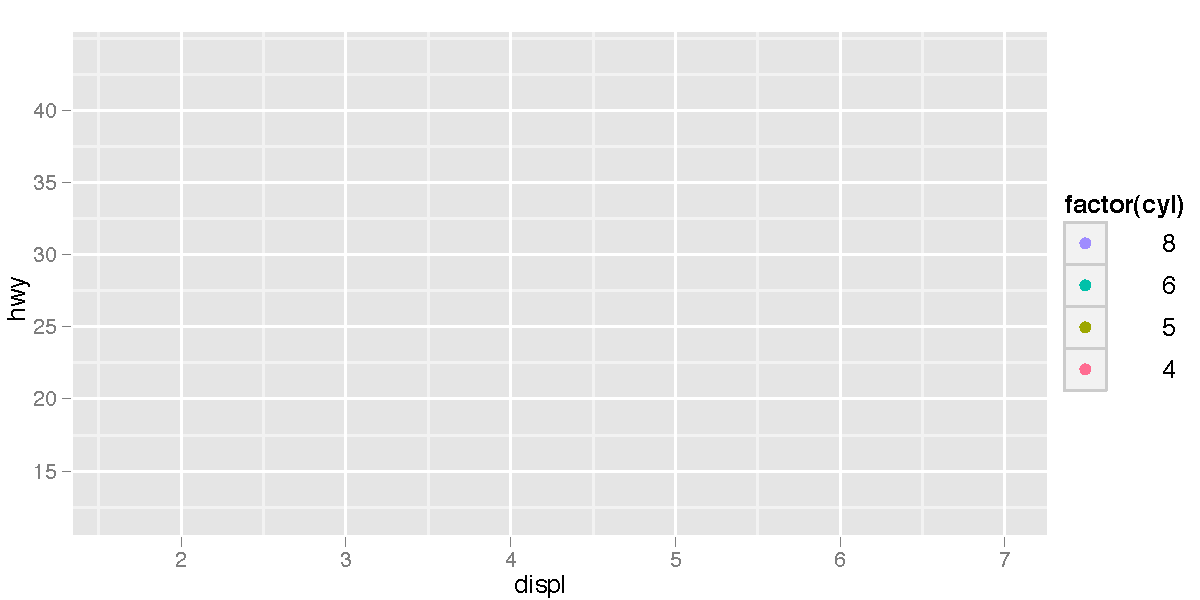
\includegraphics[width=0.8\linewidth]{diagrams/empty}
  \caption{Contributions from the scales, the axes and legend and grid lines, and the plot background.  Contributions from the data, the point geom, have been removed.}
  \label{fig:empty}
\end{figure}

\hyperdef{}{sec:complex-plot}{\section{Adding
complexity}\label{sec:complex-plot}}

With a simple example under our belts, let's now turn to look at the
slightly more complicated plot in Figure \ref{fig:complex}. This plot
adds three new components to the mix: facets, multiple layers and
statistics. The facets and layers expand the data structure described
above: each facet panel in each layer has its own dataset. You can think
of this as a 3d array: the panels of the facets form a 2d grid, and the
layers extend upwards in the 3rd dimension. In this case the data in the
layers is the same, but in general we can plot different datasets on
different layers. Table \ref{tbl:data-complex} shows the first few rows
of the data in each facet.

\begin{Shaded}
\begin{Highlighting}[]
\KeywordTok{qplot}\NormalTok{(displ, hwy, }\DataTypeTok{data=}\NormalTok{mpg, }\DataTypeTok{facets =} \NormalTok{. ~}\StringTok{ }\NormalTok{year) +}\StringTok{ }\KeywordTok{geom_smooth}\NormalTok{()}
\end{Highlighting}
\end{Shaded}

\begin{figure}

{\centering \includegraphics[width=\linewidth]{figures/masterycomplex-1} 

}

\caption{A more complex plot with facets and multiple layers.\label{fig:complex}}
\end{figure}

\begin{table}[ht]
\centering
\begin{tabular}{rrrrrr}
  \hline
x & y & colour & x & y & colour \\ 
  \hline
1.80 &  29 &   4 & 2.00 &  31 &   4 \\ 
  1.80 &  29 &   4 & 2.00 &  30 &   4 \\ 
  2.80 &  26 &   6 & 3.10 &  27 &   6 \\ 
  2.80 &  26 &   6 & 2.00 &  28 &   4 \\ 
  1.80 &  26 &   4 & 2.00 &  27 &   4 \\ 
  1.80 &  25 &   4 & 3.10 &  25 &   6 \\ 
  2.80 &  25 &   6 & 3.10 &  25 &   6 \\ 
  2.80 &  25 &   6 & 3.10 &  25 &   6 \\ 
  2.80 &  24 &   6 & 4.20 &  23 &   8 \\ 
  5.70 &  17 &   8 & 5.30 &  20 &   8 \\ 
   \hline
\end{tabular}
\caption{A 1 $\times$ 2 grid of data frames used for faceting.  In general, this structure also has a third dimension for layers, but in this example the data for each layer is the same.} 
\label{tbl:data-complex}
\end{table}

The smooth layer is different to the point layer because it doesn't
display the raw data, but instead displays a statistical transformation
of the data. Specifically, the smooth layer fits a smooth line through
the middle of the data. This requires an additional step in the process
described above: after mapping the data to aesthetics, the data is
passed to a statistical transformation, or \textbf{stat}, which
manipulates the data in some useful way. In this example, the stat fits
the data to a loess smoother, and then returns predictions from evenly
spaced points within the range of the data. Other useful stats include 1
and 2d binning, group means, quantile regression and contouring.

As well as adding an additional step to summarise the data, we also need
some extra steps when we get to the scales. This is because we now have
multiple datasets (for the different facets and layers) and we need to
make sure that the scales are the same across all of them. Scaling
actually occurs in three parts: transforming, training and mapping. We
haven't mentioned transformation before, but you have probably seen it
before in log-log plots. In a log-log plot, the data values are not
linearly mapped to position on the plot, but are first log-transformed.

\begin{itemize}
\item
  Scale transformation occurs before statistical transformation so that
  statistics are computed on the scale-transformed data. This ensures
  that a plot of \(\log(x)\) vs. \(\log(y)\) on linear scales looks the
  same as \(x\) vs. \(y\) on log scales. There are many different
  transformations that can be used, including taking square roots,
  logarithms and reciprocals. See
  \hyperref[ssub:scale-continuous]{continuous scales} for more details.
\item
  After the statistics are computed, each scale is trained on every
  dataset from all the layers and facets. The training operation
  combines the ranges of the individual datasets to get the range of the
  complete data. Without this step, scales could only make sense locally
  and we wouldn't be able to overlay different layers because their
  positions wouldn't line up. Sometimes we do want to vary position
  scales across facets (but never across layers), and this is described
  more fully in \hyperref[sub:controlling-scales]{controlling scales}.
\item
  Finally the scales map the data values into aesthetic values. This is
  a local operation: the variables in each dataset are mapped to their
  aesthetic values producing a new dataset that can then be rendered by
  the geoms.
\end{itemize}

Figure \ref{fig:schematic} illustrates the complete process
schematically.

\begin{figure}[htbp]
  \centering
  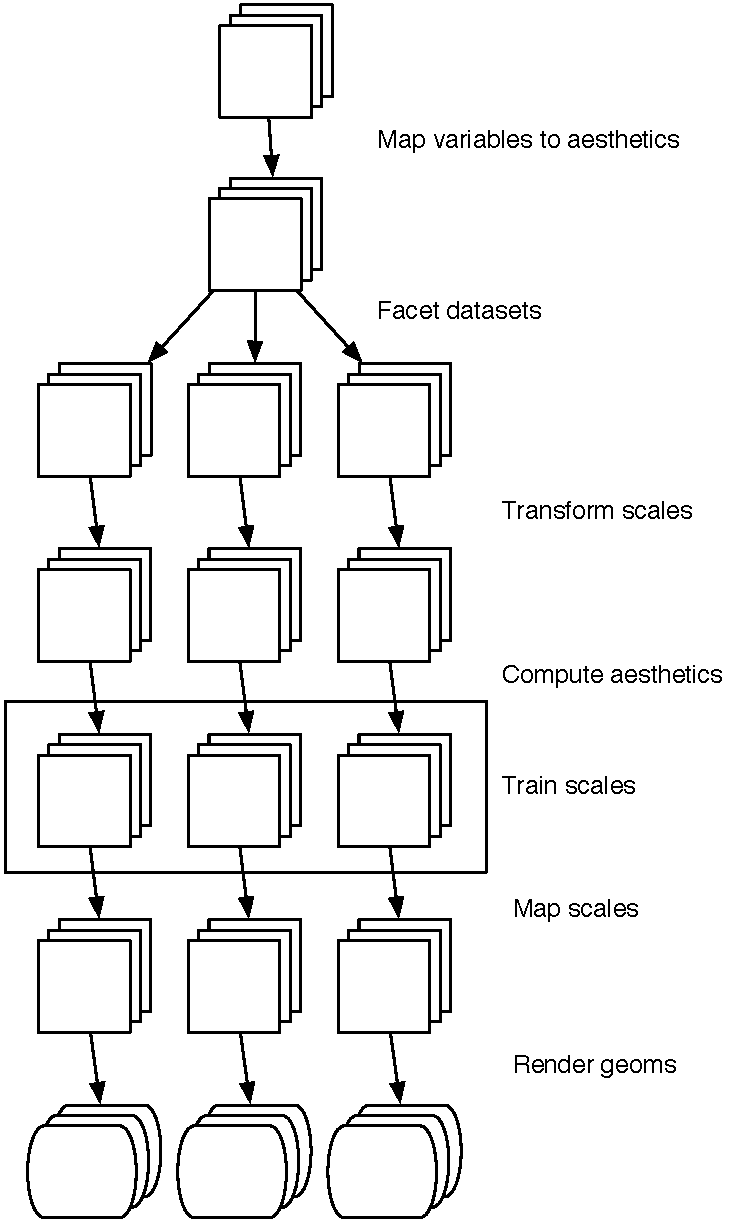
\includegraphics[width=4in]{diagrams/mastery-schema}
  \caption{Schematic description of the plot generation process. Each square represents a layer, and this schematic represents a plot with three layers and three panels. All steps work by transforming individual data frames, except for training scales which doesn't affect the data frame and operates across all datasets simultaneously.}
  \label{fig:schematic}
\end{figure}

\hyperdef{}{sec:components}{\section{Components of the layered
grammar}\label{sec:components}}

In the examples above, we have seen some of the components that make up
a plot, data and aesthetic mappings, geometric objects (geoms),
statistical transformations (stats), scales and faceting. We have also
touched on the coordinate system. One thing we didn't mention is the
position adjustment, which deals with overlapping graphic objects.
Together, the data, mappings, stat, geom and position adjustment form a
\textbf{layer}. A plot may have multiple layers, as in the example where
we overlaid a smoothed line on a scatterplot. All together, the layered
grammar defines a plot as the combination of: \index{Grammar!components}

\begin{itemize}
\itemsep1pt\parskip0pt\parsep0pt
\item
  A default dataset and set of mappings from variables to aesthetics.
\item
  One or more layers, each composed of a geometric object, a statistical
  transformation, and a position adjustment, and optionally, a dataset
  and aesthetic mappings.
\item
  One scale for each aesthetic mapping.
\item
  A coordinate system.
\item
  The faceting specification.
\end{itemize}

The following sections describe each of the higher level components more
precisely, and point you to the parts of the book where they are
documented.

\subsection{Layers}

\textbf{Layers} are responsible for creating the objects that we
perceive on the plot. A layer is composed of four parts:
\index{Layers!components}

\begin{itemize}
\itemsep1pt\parskip0pt\parsep0pt
\item
  data and aesthetic mapping,
\item
  a statistical transformation (stat),
\item
  a geometric object (geom)
\item
  and a position adjustment.
\end{itemize}

The properties of a layer are described in \hyperref[cha:layers]{layers}
and how they can be used to visualise data in
\hyperref[cha:toolbox]{toolbox}.

\subsection{Scales}\label{sub:scales}

A \textbf{scale} controls the mapping from data to aesthetic attributes,
and we need a scale for every aesthetic used on a plot. Each scale
operates across all the data in the plot, ensuring a consistent mapping
from data to aesthetics. Some scales are illustrated in Figure
\ref{fig:scales}.

\begin{figure}

{\centering \includegraphics[width=4in]{figures/masteryscales-1} 

}

\caption{Examples of legends from four different scales. From left to right: continuous variable mapped to size, and to colour, discrete variable mapped to shape, and to colour. The ordering of scales seems upside-down, but this matches the labelling of the $y$-axis: small values occur at the bottom.\label{fig:scales}}
\end{figure}

A scale is a function, and its inverse, along with a set of parameters.
For example, the colour gradient scale maps a segment of the real line
to a path through a colour space. The parameters of the function define
whether the path is linear or curved, which colour space to use (e.g.,
LUV or RGB), and the colours at the start and end.

The inverse function is used to draw a guide so that you can read values
from the graph. Guides are either axes (for position scales) or legends
(for everything else). Most mappings have a unique inverse (i.e., the
mapping function is one-to-one), but many do not. A unique inverse makes
it possible to recover the original data, but this is not always
desirable if we want to focus attention on a single aspect.

For more details, see the \hyperref[cha:scales]{scales chapter}

\subsection{Coordinate system}\label{sub:coordinate-systems}

A coordinate system, or \textbf{coord} for short, maps the position of
objects onto the plane of the plot. Position is often specified by two
coordinates \((x, y)\), but potential could be three or more (although
this is not yet implemented in \textbf{ggplot}). The Cartesian
coordinate system is the most common coordinate system for two
dimensions, while polar coordinates and various map projections are used
less frequently. \index{Coordinate systems!introduction}

Coordinate systems affect all position variables simultaneously and
differ from scales in that they also change the appearance of the
geometric objects. For example, in polar coordinates, bar geoms look
like segments of a circle. Additionally, scaling is performed before
statistical transformation, while coordinate transformations occur
afterward. The consequences of this are shown in
\hyperref[sub:coord-transformation]{coordinate transformations}.

Coordinate systems control how the axes and grid lines are drawn. Figure
\ref{fig:coord} illustrates three different types of coordinate systems.
Very little advice is available for drawing these for non-Cartesian
coordinate systems, so a lot of work needs to be done to produce
polished output. See \hyperref[sec:coord]{coordinate systems} for more
details.

\begin{figure}

{\centering \includegraphics[width=0.32\linewidth]{figures/masterycoord-1} \includegraphics[width=0.32\linewidth]{figures/masterycoord-2} \includegraphics[width=0.32\linewidth]{figures/masterycoord-3} 

}

\caption{Examples of axes and grid lines for three coordinate systems: Cartesian, semi-log and polar. The polar coordinate system illustrates the difficulties associated with non-Cartesian coordinates: it is hard to draw the axes well.\label{fig:coord}}
\end{figure}

\subsection{Faceting}\label{sub:intro-faceting}

There is also another thing that turns out to be sufficiently useful
that we should include it in our general framework: faceting, a general
case of the conditioned or trellised plots. This makes it easy to create
small multiples each showing a different subset of the whole dataset.
This is a powerful tool when investigating whether patterns hold across
all conditions. The faceting specification describes which variables
should be used to split up the data, and whether position scales should
be free or constrained. Faceting is described in
\hyperref[cha:position]{position}.

\hyperdef{}{sec:data-structures}{\section{Data
structures}\label{sec:data-structures}}

This grammar is encoded into R data structures in a fairly
straightforward way. A plot object is a list with components
\texttt{data}, \texttt{mapping} (the default aesthetic mappings),
\texttt{layers}, \texttt{scales}, \texttt{coordinates} and
\texttt{facet}. The plot object has one other component we haven't
discussed yet: \texttt{options}. This is used to store the plot-specific
theme options described in \hyperref[cha:polishing]{Polishing}.
\index{ggplot!data structures}

Plots can be created in two ways: all at once with \texttt{qplot()}, as
shown in the previous chapter, or piece-by-piece with \texttt{ggplot()}
and layer functions, as described in the next chapter. Once you have a
plot object, there are a few things you can do with it:

\begin{itemize}
\item
  Render it on screen, with \texttt{print()}. This happens automatically
  when running interactively, but inside a loop or function, you'll need
  to \texttt{print()} it yourself. \indexf{print}
\item
  Render it to disk, with \texttt{ggsave()}, described in
  \hyperref[sec:saving]{saving your output}.
\item
  Briefly describe its structure with \texttt{summary()}.
  \indexf{summary}
\item
  Save a cached copy of it to disk, with \texttt{save()}. This saves a
  complete copy of the plot object, so you can easily re-create that
  exact plot with \texttt{load()}. Note that data is stored inside the
  plot, so that if you change the data outside of the plot, and then
  redraw a saved plot, it will not be updated. \indexf{save}
  \indexf{load}
\end{itemize}

The following code illustrates some of these tools.

\begin{Shaded}
\begin{Highlighting}[]
\NormalTok{p <-}\StringTok{ }\KeywordTok{qplot}\NormalTok{(displ, hwy, }\DataTypeTok{data =} \NormalTok{mpg, }\DataTypeTok{colour =} \KeywordTok{factor}\NormalTok{(cyl))}
\KeywordTok{summary}\NormalTok{(p)}
\CommentTok{#> data: manufacturer, model, displ, year, cyl, trans,}
\CommentTok{#>   drv, cty, hwy, fl, class [234x11]}
\CommentTok{#> mapping:  colour = factor(cyl), x = displ, y = hwy}
\CommentTok{#> faceting: facet_null() }
\CommentTok{#> -----------------------------------}
\CommentTok{#> geom_point:  }
\CommentTok{#> stat_identity:  }
\CommentTok{#> position_identity: (width = NULL, height = NULL)}
\end{Highlighting}
\end{Shaded}

\begin{Shaded}
\begin{Highlighting}[]
\CommentTok{# Save plot object to disk}
\KeywordTok{save}\NormalTok{(p, }\DataTypeTok{file =} \StringTok{"plot.rdata"}\NormalTok{)}
\CommentTok{# Load from disk}
\KeywordTok{load}\NormalTok{(}\StringTok{"plot.rdata"}\NormalTok{)}
\CommentTok{# Save png to disk}
\KeywordTok{ggsave}\NormalTok{(}\StringTok{"plot.png"}\NormalTok{, }\DataTypeTok{width =} \DecValTok{5}\NormalTok{, }\DataTypeTok{height =} \DecValTok{5}\NormalTok{)}
\end{Highlighting}
\end{Shaded}

Wickham, Hadley. 2008. ``Practical Tools for Exploring Data and
Models.'' PhD thesis, Iowa State University.
\url{http://had.co.nz/thesis}.

Wilkinson, Leland. 2005. \emph{The Grammar of Graphics}. 2nd ed.
Statistics and Computing. Springer.
